\documentclass[11pt]{article}
\usepackage[utf8]{inputenc}
\usepackage[english]{babel}
\usepackage{bilal2vec}

\title{CS 370 - A2}
\author{Bilal Khan\\
\href{mailto:bilal2vec@gmail.com}{bilal2vec@gmail.com}}
\date{\today}

\begin{document}

\maketitle

\tableofcontents

\section{1}

Consider the initial value problem

\[ y^\prime(t) = -y^2 \cos(2t), y(0) = 1 \]

\subsection{(a)}

Show that $y(t) = \frac{2}{\sin(2t) + 2}$ is an exact closed-form solution to this particular IVP (including initial conditions). Hint: You do not need to analytically solve the ODE; just show that the proposed solution $y(t)$ satisfies it.

We can show that this is an exact solution by checking if it satisfies the ODE and the initial condition. Differentiating the proposed solution, we get

\[ y^\prime(t) = \frac{d}{dt} \left( \frac{2}{\sin(2t) + 2} \right) = \frac{-4 \cos(2t)}{(\sin(2t) + 2)^2} = -y^2 \cos(2t) \]

\[ y(0) = \frac{2}{\sin(2 (0)) + 2} = \frac{2}{0 + 2} = 1 \]

\subsection{(b)}

Create a single Jupyter notebook for the rest of this question, A2Q1.ipynb. Define a function, Dynamics(t,y) that implements the dynamics function for the above problem given t and y. i.e., it should return the corresponding derivative value $y^\prime(t)$. Define a second function ExactVal(t) that returns the exact solution of y for a given time t.

\subsection{(c)}

Define a function, y = ForwardEuler(t0, tfinal, N, y0), which takes as input the initial time, t0, the final time, tfinal, the number of steps, N, and the initial value, y0, and implements teh Forward Euler method. It should return the computed approximate solution as a vector y of length N+1, such that

\[ y_i \approx y(t_i), \forall i = 0, 1, 2, \cdots, N \]

where $t_i = t_0 + ih, h = \frac{t_{final} - t_0}{N}$ and $y(t_i)$ denotes the exact solution at time $t = t_i$. Your ForwardEuler function should call the function dynamics internally when needed.

\subsection{(d)}

Next, apply your ForwardEuler function to solve the IVP to time tfinal = 5, first with $N_1 = 20$ constant-size timesteps and then again with $N_2 = 40$ constant-size timesteps. Plot these numerical solutions together on the same graph over the doman $0 \leq t \leq 5$ using the + symbol for the first solution and the o symbol for the second solution. Also on the same graph plot the analytical solution using solid lines. (To create the exact solution plot, evaluate it at the same discrete times as the $N_2$ solution).

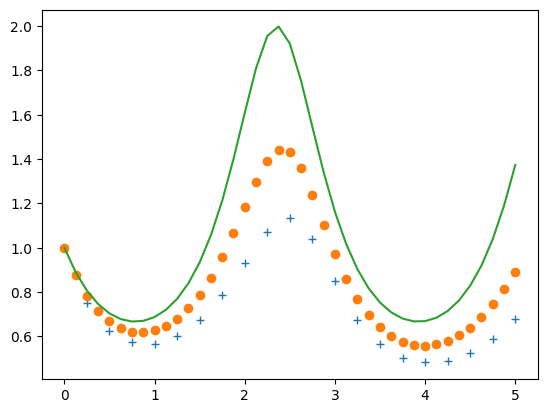
\includegraphics[width=300pt]{a2q1_1.png}

\subsection{(e)} 

A time stepping rule for another second order Runge-Kutta scheme is given by:

\begin{align*}
  k_1 &= f(t_n, y_n) \\
  k_2 &= f(t_n + 2h/3, y_n + 2hk_1/3) \\
  y_{n + 1} &= y_n + h(k_1/4 + 3k_2/4) \\
\end{align*}

Define another function, y = RK2(t0, tfinal, N, y0) which implements the Runge-Kutta method, similar to what you did in part (c) for Forward Euler.

\subsection{(f)}

Next, apply both your ForwardEuler and RK2 functions to solve the IVP to time tfinal = 5, with N = 20 constant-size time steps. Plot these two numerical solutions on the same graph over the domain $0 \leq t \leq 5$, using the + symbol for the Forward Euler solution and the o symbol for the RK2 solution. Also on the same graph, plot the analytical solution using solid lines. (To create the exact solution plot, evaluate it at the same discrete times as the other two solutions.)

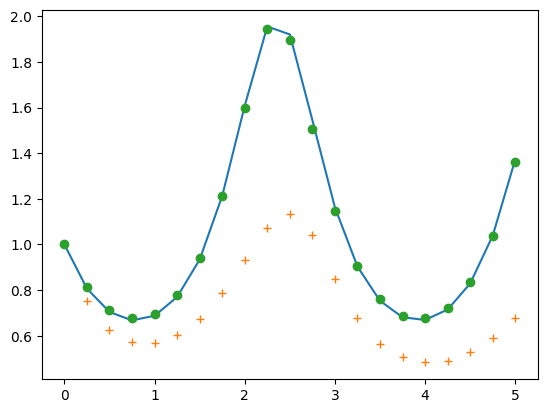
\includegraphics[width=300pt]{a2q1_2.png}


\subsection{(g)}

We would now like to calculate numerical evidence illustrating the order of the Forward Euler method. Let err(h) denote the absolute (global) error at tfinal after computing with step size h. For a p-order method, $err(h) \approx Ch^p$ for some constant $C$, and so the effect of cutting the step size in half is $\frac{err(h/2)}{err(h)} \approx \frac{1}{2^p}$ i.e., the error is reduced by a factor of $2^p$. Therefore, the order p of a given method can be illustrated by calculating the above ratios for decreasing h. For the Forward Euler method, calculate a vector of successive computed values for the solution at $t = 2$ based on cutting the step size in half a number of times. Specifically, use $N = 5 \cdot 2^i$ timesteps, for $i = 0, 1, \cdots, 9$. Your code should then calculate the errors for each timestep size and the successive ratios $err(h/2) / err(h)$, and print this information in rows in a simple text table (just use print, no fancy formatting required). From your experimental evidence, what is the order of the Forward Euler method?

From the table, we have that $1/2^p \approx 0.5$, so $p \approx 1$. Therefore, the order of the Forward Euler method is 1.

\subsection{(h)}

Repeat part (g) for the RK2 method. What is the order of this RK2 method?

From the table, we have that $1/2^p \approx 0.25$, so $p \approx 2$. Therefore, the order of the RK2 method is 2.

\section{2}

Consider Newton's equations of motin for a two-body problem specified by:

\[ \dfrac{d^2x}{dt^2} (t) = - \dfrac{x(t)}{(x(t)^2 + y(t)^2)^{3/2}} ; x(0) = 0.4; \dfrac{dx}{dt}(0) = 0 \]
\[ \dfrac{d^2y}{dt^2} (t) = - \dfrac{y(t)}{(x(t)^2 + y(t)^2)^{3/2}} ; y(0) = 0; \dfrac{dy}{dt}(0) = 2 \]

As $t$ ranges from $0$ to $2\pi$, $(x(t), y(t))$ defines an ellipse. Convert this initial value problem to an equivalent first-order system of ODEs which has the form $\dfrac{du}{dt}(t) = F(t, u)$.

We can convert this to a first-order system of ODEs by letting:

\[ u = \begin{bmatrix} x \\ y \\ \dfrac{dx}{dt} \\ \dfrac{dy}{dt} \\ \end{bmatrix} \]

Initial conditions for $u$ are then given:

\[ u(0) = \begin{bmatrix} 0.4 \\ 0 \\ 0 \\ 2 \\ \end{bmatrix} \]

\[
  \dfrac{du}{dt}(t) =
  \begin{bmatrix}
    dx/dt \\
    dy/dt \\
    d^2x/dt^2 \\
    d^2y/dt^2 \\
  \end{bmatrix}
  =
  \begin{bmatrix}
    u_3(t) \\
    u_4(t) \\
    - \dfrac{u_1(t)}{(u_1(t)^2 + u_2(t)^2)^{3/2}} \\
    - \dfrac{u_2}{(u_1(t)^2 + u_2(t)^2)^{3/2}} \\
  \end{bmatrix}
\]

\section{3}

Solve the initial value problem by hand calculations

\[ f(x, y) = \dfrac{dy(x)}{dx} = x + y, y(0) = 2 \]

using Forward Euler and Improved Euler methods with step size $h = 0.5$. Show your work. Compare your results with the exact solution $y(x) = 3e^x - x - 1$ at $x = 0.5$ and $1$. Compute the errors of the approximate solutions given by these methods. (You may use a calculator to perform the individual arithmetic steps, but be sure to show how you arrived at your result. You are not allowed to write Python code for this question.) Display your results in a table which shows the solutions given by the ODE methods and their corresponding errors at each time step.

\begin{align*}
  y(0) &= 2 \\
  y(0.5) &= 3e^{0.5} - 0.5 - 1 = 3.45 \\
  y(1) &= 3e^1 - 1 - 1 = 6.15 \\
  y(0.5) &\approx y(0) + 0.5 \cdot f(0, 2) \\
  &= 2 + 0.5 \cdot (0 + 2) = 3 \\
  y(1) &\approx y(0.5) + 0.5 \cdot f(0.5, 3) \\
  &= 3 + 0.5 \cdot (0.5 + 3) = 4.75 \\
  y(0.5) &\approx y(0) + \frac{0.5}{2} \left( f(0, 2) + f(0.5, y(0) + 0.5 \cdot f(0, 2)) \right) \\
  &= 2 + 0.25 (2 + 0.5 + 2 + 0.5 \cdot (2 + 0)) \\
  &= 2 + 0.25 (2 + 2 + 0.5 + 0.5 (2)) = 2 + 0.25 (2 + 2 + 1 + 0.5) \\
  &= 2 + 0.25 (5.5) = 2 + 1.375 = 3.375 \\
  y(1) &\approx y(0.5) + \frac{0.5}{2} \left( f(0.5, 3.375) + f(1, y(0.5) + 0.5 \cdot f(0.5, 3.375)) \right) \\
  &= 3.375 + 0.25 (0.5 + 3.375 + 1 + 3.375 + 0.5 (0.5 + 3.375)) \\
  &= 3.375 + 0.25 (0.5 + 3.375 + 1 + 3.375 + 0.5 (3.875)) \\
  &= 3.375 + 0.25 (0.5 + 3.375 + 1 + 3.375 + 1.9375) \\
  &= 3.375 + 0.25 (10.1875) \\
  &= 5.92 \\
\end{align*}

\begin{table}[h]
  \centering
  \begin{tabular}{|c|c|c|c|c|c|}
      \hline
      $x$ & Exact Solution & Forward Euler & Forward Euler Error & Improved Euler & Improved Euler Error \\
      \hline
      $0$ & 2 & 2 & 0 & 2 & 0 \\
      $0.5$ & 3.45 & 3 & 0.45 & 3.375 & 0.075 \\
      $1$ & 6.15 & 4.75 & 1.4 & 5.92 & 0.23 \\
      \hline
  \end{tabular}
\end{table}

\section{4}

Consider solving a differential equation $y^\prime(t) = f(t,y(t))$ using the time-stepping method given by

\[ \dfrac{y_{n+1} - y_{n-1}}{2} = h f(t_n, y_n) \]

The timestep is a constant $h = t_{n+1} - t_n = t_n - t_{n-1}$

\subsection{(a)}

State whether this method is explicit or implicit

This is an explicit method since we can calculate $y_{n+1}$ directly in terms of $t_n, t_{n-1}, y_n, y_{n-1}$: $y_{n+1} = 2hf(t_n, y_n) + y_{n-1}$

\subsection{(b)}

State whether this is a single-step or multi-step method

Multi-step, because we need $y_n$ and $y_{n-1}$ to calculate $y_{n+1}$

\subsection{(c)}

Determine the local truncation error thos this method in the form of

\[ LTE = Ch^\alpha y^(\beta) (t_n) + O(h^{\alpha + 1}) \]

Where $C$ is a constant, and $\alpha, \beta$ are integers. Determine the values of $C, \alpha, \beta$.

\begin{align*}
  LocErr &= y_{n+1} - (y_{n-1} + 2h y^\prime_n) \\
  y_{n+1} &= y_{n} + y^\prime_{n} h + \frac{h^2}{2} y^{\prime\prime}_{n} + \frac{h^3}{6} y^{\prime\prime\prime}_{n} + O(h^4) \\
  LocErr &= y_{n} + y^\prime_{n} h + \frac{h^2}{2} y^{\prime\prime}_{n} + \frac{h^3}{6} y^{\prime\prime\prime}_{n} + O(h^4) - (y_{n-1} + 2hy^{\prime}_n) \\
\end{align*}

\section{5}

Consider solving a differential equation $y^\prime(t) = f(t, y(t))$ using a second-order Runge-Kutta method given by

\[ y_{n+1} = y_n + \dfrac{h}{4} \left( f(t_n, y_n) + 3f \left( t_n + \dfrac{2h}{3}, y_n + \dfrac{2h}{3} f(t_n, y_n) \right) \right) \]

Analyze the stability of this method with our usual test equation

\[ f(t, y(t)) = - \lambda y(t); \lambda > 0 \]

Explain whether (and under which conditions) the method is stable

\begin{align*}
  y_{n+1} &= y_n + \dfrac{h}{4} \left( f(t_n, y_n) + 3f \left( t_n + \dfrac{2h}{3}, y_n + \dfrac{2h}{3} f(t_n, y_n) \right) \right) \\
  &= y_n + \dfrac{h}{4} \left( -\lambda y_n + 3 (-\lambda) \left( y_n + \dfrac{2h}{3} (-\lambda y_n) \right) \right) \\
  &= y_n + \dfrac{h}{4} \left( -\lambda y_n - 3 \lambda \left( y_n - \dfrac{2h}{3} \lambda y_n  \right) \right) \\
  &= y_n + \dfrac{h}{4} \left( -\lambda y_n - 3 \lambda y_n + 2h \lambda^2 y_n \right) \\
  &= y_n + \dfrac{h}{4} \left( - 4 \lambda y_n + 2h \lambda^2 y_n \right) \\
  &= y_n - h \lambda y_n + \dfrac{h^2}{2} \lambda^2 y_n \\
  &= y_n (1 - h \lambda + \dfrac{h^2}{2} \lambda^2) \\
\end{align*}

The method is stable when $|1 - h \lambda + \dfrac{1}{2} (h\lambda)^2| \leq 1$.

\section{6}

A pursuit problem involves a target and a pursuer, the latter moving in such a manner that its direction of motion is always towards the target. Figure 1 shows the trajectories of the target (CD) and the pursuer (AB):

The pursuit problem is to determine the trajectory of the pursuer, given the initial position of the pursuer and the postion vector of the target as a function of time for $t \geq 0$. Sepcifically, the trajectory of the target is prepresented by a parameter curve with parameter $t$:

\[ T(t) = (x_T(t), y_T(t), z_T(t)) \]

where $x_T(t), y_T(t), z_T(t)$ are known functions which describe the path of the target. The trajectory of the pursuer is the parameteric curve: $P(t) = (x_P(t), y_P(t), z_P(t))$. Our model of the pursuit strategy is as follows:

\begin{enumerate}
  \item At any time $t$, the motion of the pursuer must point directly to the target.
  \item The speed of the pursuer is assumed to be a known constant $s_P$.
\end{enumerate}

The implication of point (1) is that the velocity vectory at $P(t)$ should have direction $T(t) - P(t)$ at every time $t$. Notice the length of $T(t) = P(t)$ is

\[ dist(t) = \sqrt{(x_T(t) - x_P(t))^2 + (y_T(t) - y_P(t))^2 + (z_T(t) - z_P(t))^2} \]

Thus point (1) implies that $\frac{dP(t)}{dt}$ should have the direction of the unit vector $(T(t) - P(t)) / dist(t)$. On the other hand, point (2) implies that the length of $\frac{dP(t)}{dt}$ is $s_P$. Consequently, the equations describing the pursuer's motion are given by the following systems of ODEs:

\begin{align*}
  \dfrac{dx_P(t)}{dt} (t) &= \dfrac{s_P}{dist(t)} (x_T(t) - x_P(t)) \\
  \dfrac{dy_P(t)}{dt} (t) &= \dfrac{s_P}{dist(t)} (y_T(t) - y_P(t)) \\
  \dfrac{dz_P(t)}{dt} (t) &= \dfrac{s_P}{dist(t)} (z_T(t) - z_P(t)) \\
\end{align*}

The starting position of the pursuer; i.e the initial value of $P(0)$ is assumed to be known.

Solve the pursuit problem numerically using Python ODE solvers RK23 and RK45. (You may find scipy.integrate.solveivp useful). In particular, complete the Python notebook A2Q6.ipynb (download from Crowdmark) which includes the following functions

\begin{enumerate}
  \item target: The trajectory of the target is a helix which is given by:
  
  \[ x_T(t) = \sin(t), y_T(t) = \cos(t), z_T(t) = t \]

  \item rocket: This is the dynamics function of the system of the OdES for the pursuit problem. It may call the target function above.
  \item rocket events: This the event function which detects whether the purseuer has caught the target. More preceisely, you should stop the ODE solver when the distance between the pursuer and the target is less that DMIN.
  \item animate: This is for animation (you do not need to do anything)
\end{enumerate}

In the main program, you should set the time span to be $[0, 15]$, the initial position $P(0) = (0, 0, -3)$, and $DMIN=0.1$. Set the ODE options: absolute tolerance = $1e-5$, relative tolerance = $1e-5$, initial step size = $1$, maximum step size = $1$, and terminal = True when an even occurs. Also set args=(SP, DMIN) when you call the ODE solver.

Use different speeds, $SP = 1.4, 1.5, 1.6, 1.7$ to solve the problem. For each speed, do the following

\subsection{(a)} Solve the pursuit problem using RK23 and RK45 using the parameters described above

\subsection{(b)} Report (1) the number of time steps used by the RK23 and RK45, (2) the number of evaluations of the right-hand side, and (3) the time of intercept if the pursuer and the target intercept; otherwise, report no intercept.

\begin{table}[h]
  \centering
  \begin{tabular}{c|ccc|ccc}
  \hline
  $SP$ & \multicolumn{3}{c|}{RK23} & \multicolumn{3}{c}{RK45} \\
   & Steps & Evaluations & Intercept & Steps & Evaluations & Intercept \\
  \hline
  $1.4$ & $153$ & $463$ & N/A & $36$ & $14650$ & $12.54$ \\
  $1.5$ & $4871$ & $14650$ & $12.54$ & $2934$ & $1713$ & $12.54$ \\
  $1.6$ & $34772$ & $104350$ & $8.28$ & $16901$ & $101569$ & $8.27$ \\
  $1.7$ & $59364$ & $178141$ & $6.32$ & $26523$ & $167185$ & $6.32$ \\
  \hline
  \end{tabular}
\end{table}
    
  
\subsection{(c)} Make a subplot of the target and pursuer trajectories given by RK23 and another subplot by RK45, Label the axes and the title should include the speed and the name of the solver.

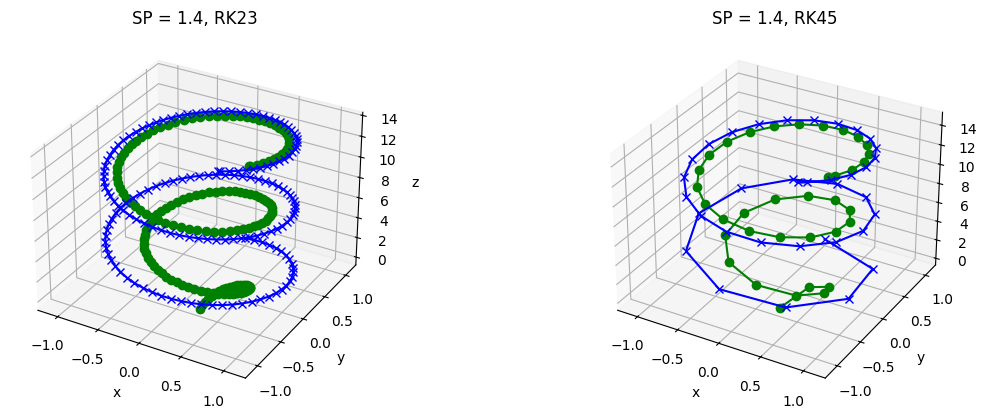
\includegraphics[width=300pt]{a2q6_1.png}

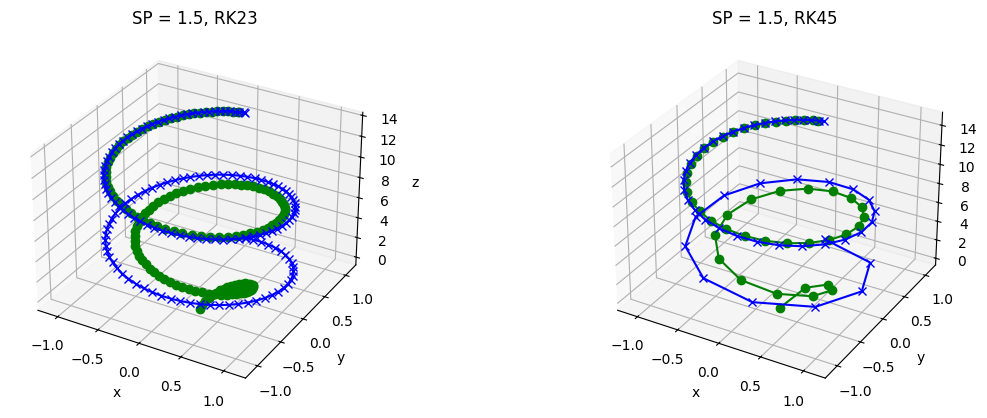
\includegraphics[width=300pt]{a2q6_2.png}

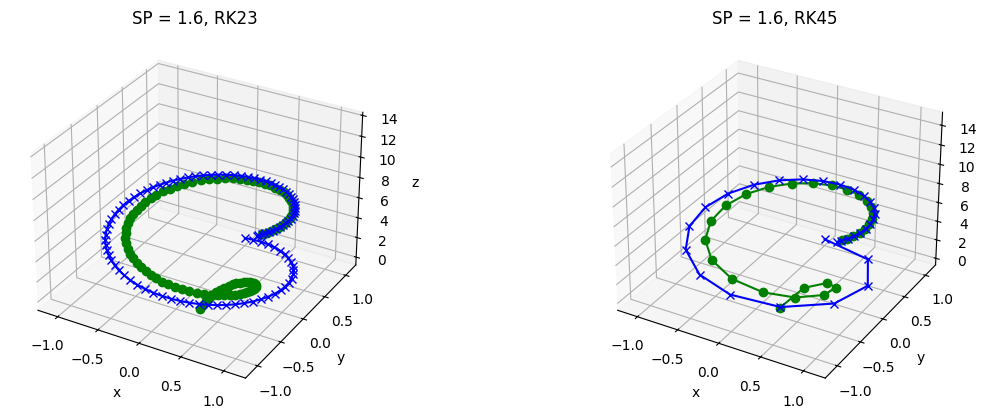
\includegraphics[width=300pt]{a2q6_3.png}

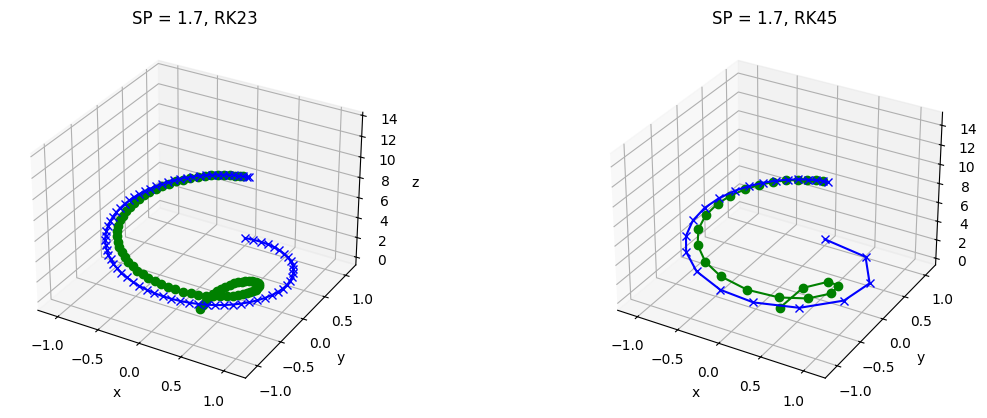
\includegraphics[width=300pt]{a2q6_4.png}

\subsection{(d)}

Which of the ODE solver is more efficient? Explain your answer by commenting on the number of timesteps and function evaluations.

RK45 is more efficient. It uses fewer steps and fewer function evaluations.


\end{document}
